\chapter{Modelling VRP in Constraint Programming}
\section{Input Data and any Potential Data Processing}
Let N the number of customers, input data are as follow:
\begin{enumerate}
    \item \begin{math}locX_{i}\end{math} for each i in \{1..N+1\} with a float domain defines the coordinate X of a location \begin{math}L_{i}\end{math}, the last one is a reference of the depot coordinate 
    \item \begin{math}locY_{i}\end{math} for each i in \{1..N+1\} with a float domain defines the coordinate Y of a location, the last one is a reference of the depot coordinate
    \item a list \begin{math}[de_{1}, ..., de_{N}]\end{math} with \begin{math}d_{i}, i \in \{1..N\}\end{math} the demand of the customer i
    \item V is the number of vehicles available
    \item a list \begin{math}[c_{1},..., c_{V}]\end{math} with \begin{math} c_{i}, i \in \{1..V\}]\end{math} the capacity of the vehicle i
\end{enumerate}
To solve the problem, each location need to be visited. Therefore, it's important to take trace of visits in the routes of a solution. Each node is represent a visit checked by only one vehicle. 
From the initial set of input data and observations taken from the problem, it's necessary to define following processing data, useful to establish constraints in the model or clarify some types of values:
\begin{enumerate}
 \setcounter{enumi}{5}
    \item \begin{math}NumVisits\end{math} is the total number of visits of the final combined route. It is equal to \begin{math}N + V * 2\end{math}
    \item list of \begin{math}d= [d_{1,1},d_{1,2},..., d_{N,N}, d_{1,N+1},...,d_{N+V*2,N+V*2}] \end{math} represents distances between two nodes. Values are calculated as follow:\newline
    \begin{enumerate}
        \item\begin{math}\forall i,j \in \{1,...,N\}: d_{ij} = \sqrt{(locX_{j} - locX_{i})^2 + (locY_{j} - locY_{i})^2} * 1000\end{math}
        \item\begin{math}\forall i \in \{1,...,N\}, j \in \{N + 1,...,  N + V * 2\}:\newline d_{ij} = \sqrt{(locX_{N+1} - locX_{i})^2 + (locY_{N+1} - locY_{i})^2} * 1000\end{math}
        \item \begin{math}\forall i,j \in \{N + 1,...,  N + V * 2\}: d_{i,j} = 0\end{math}
    \end{enumerate}
    \item A weight of vehicle \begin{math}w\end{math} with integer domain represent the relevance of the minimizing the number of vehicles respects the minimal distance traveled during the optimal research. 
\end{enumerate}
\section{Decision Variables}
A solution of the problem is made up of routes, one route for vehicles. It is a sequence of nodes (visits) formed by customers nodes (visited in the route) and 2 depot visits (one start and one end node).

\begin{figure}[h]
    \centering
    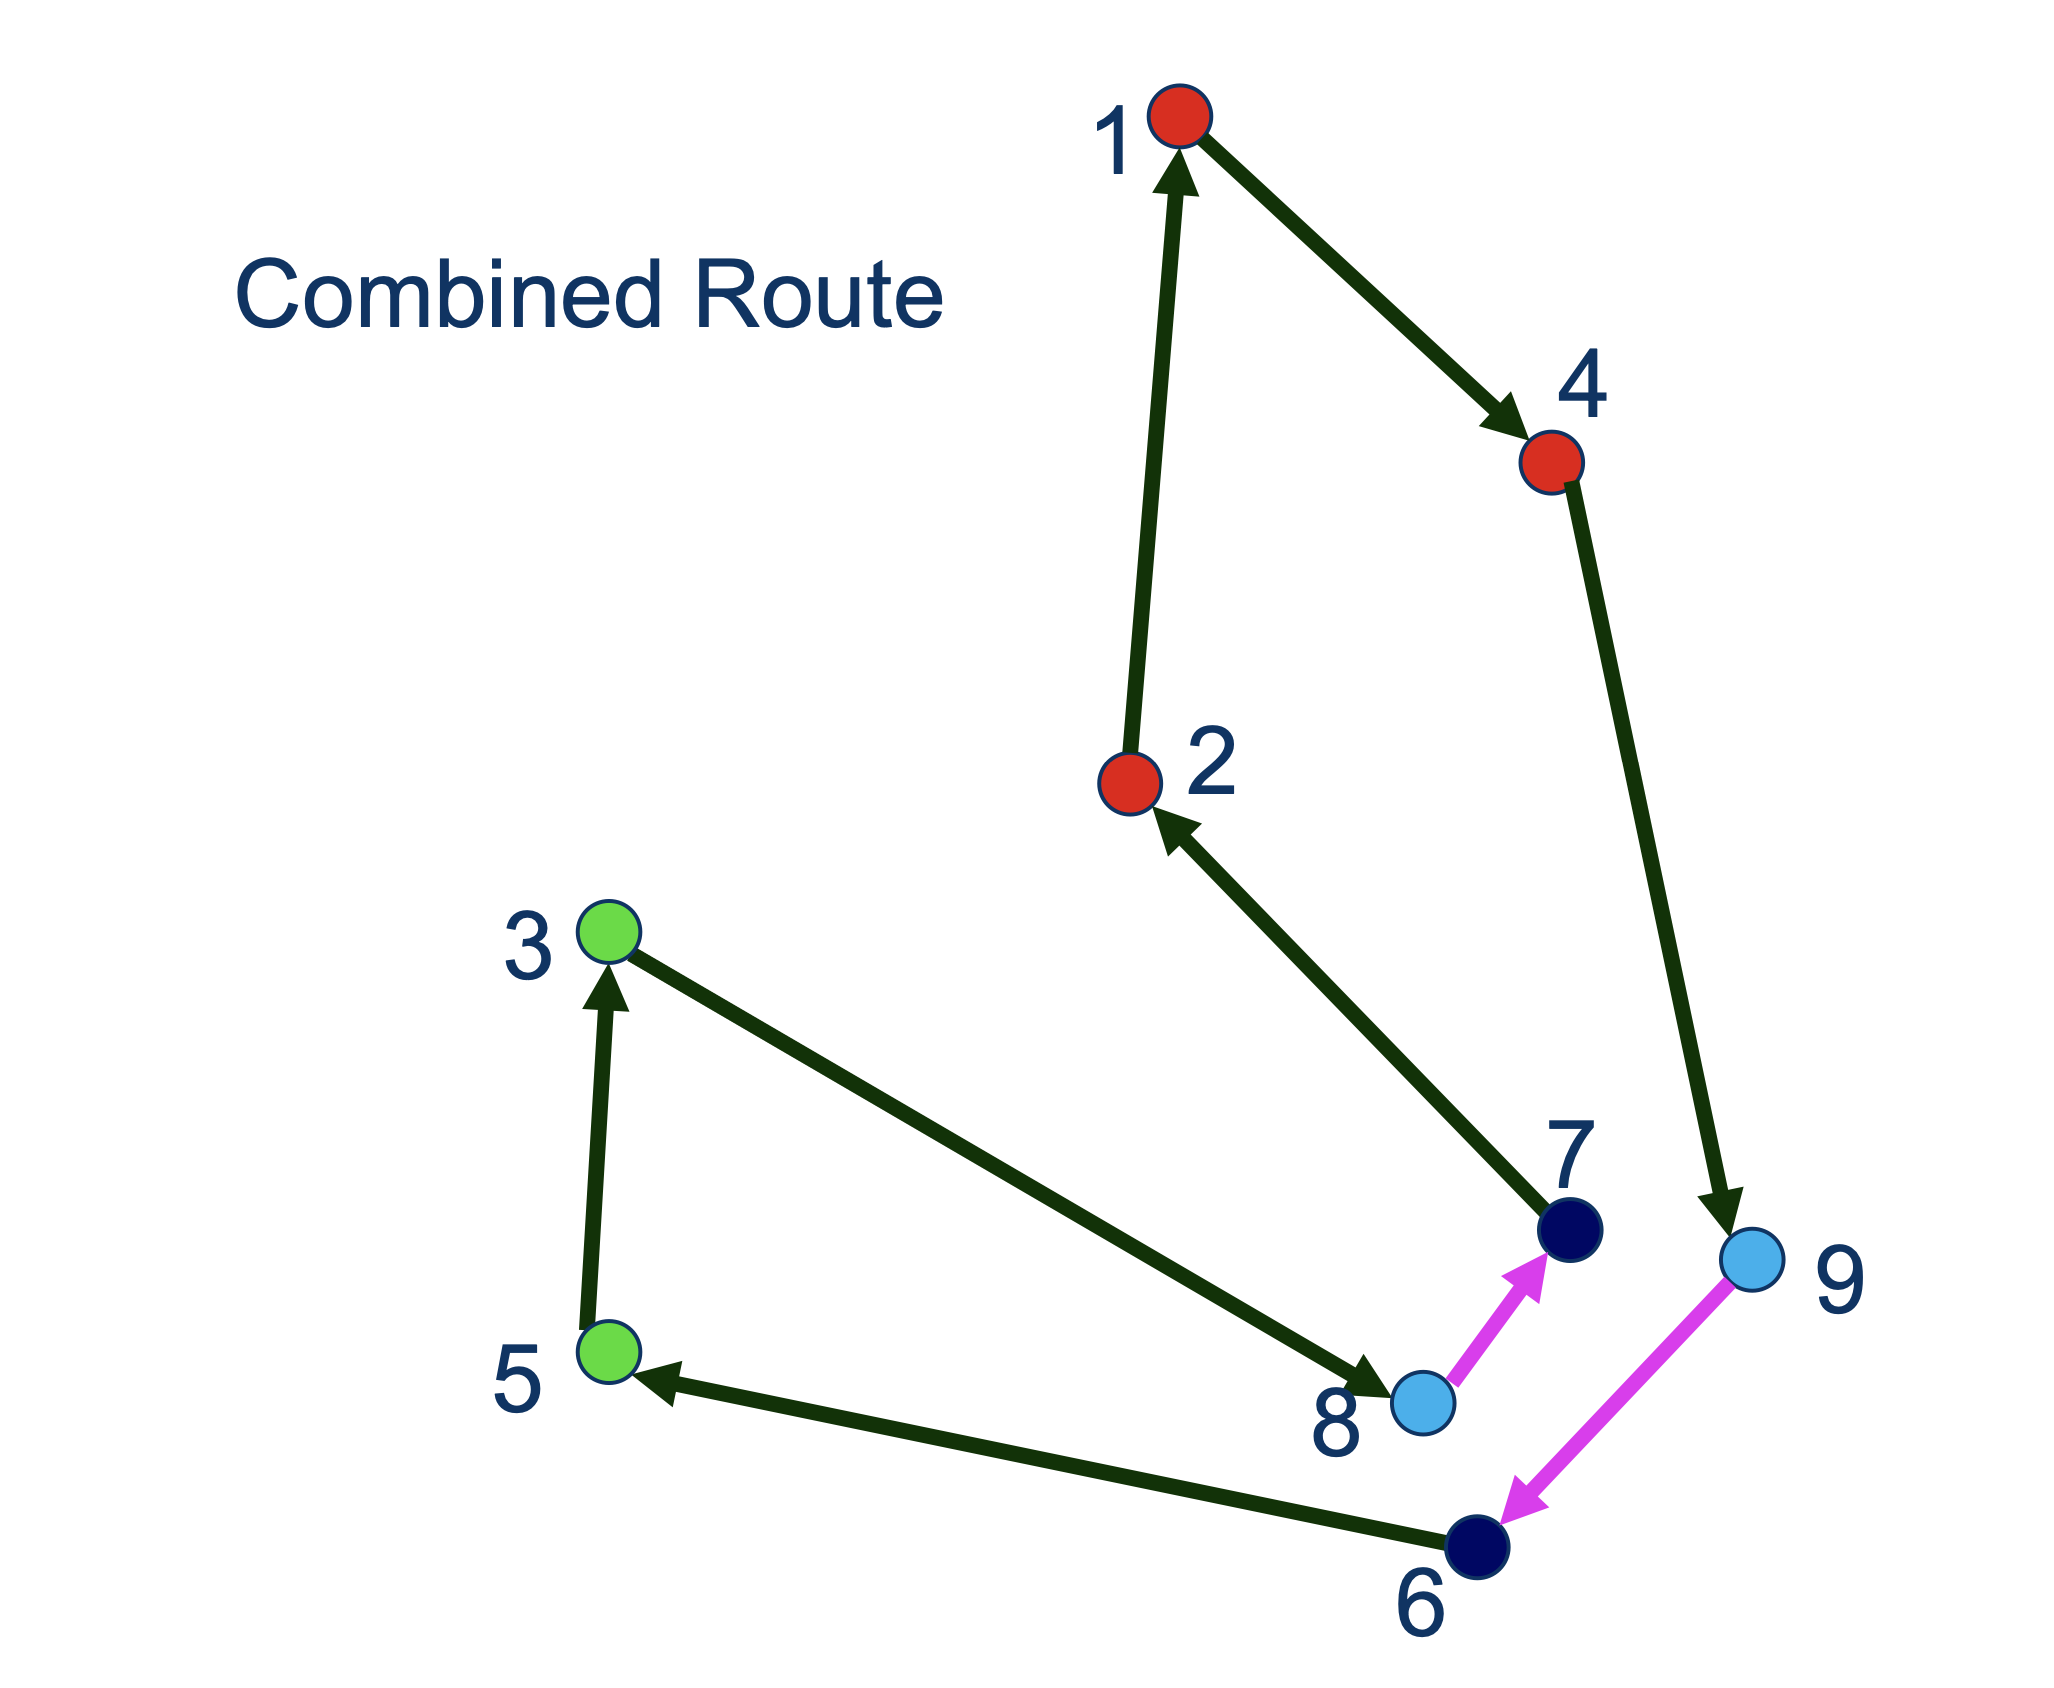
\includegraphics[width=0.5\textwidth]{images/combined-route-solution.png}
    \caption{A solution of VRP with 5 customers and 2 vehicles with 2 routes. Nodes 6,7 are start visits nodes 9,8 are end visits and represents the same location: the depot}
    \label{fig:mesh1}
\end{figure}

Starting from these observations, the model has the following decision variables:
\begin{enumerate}
    \item list of vehicles assignments \begin{math}ve = [ve_{1}, ..., ve_{NumVisits}] \end{math} with domains \begin{math}\{1,...,V\}\end{math}where for each \begin{math}i \in \{1,..., NumVisits\}, j \in {1,...,V} ,\end{math}if \begin{math} ve_{i} = j\end{math} then the node i is visited by the vehicle j
    \item list of successions \begin{math}s=[s_{1},...,s_{NumVisits}]\end{math} in the combined route with domains \begin{math}\{1,..., NumVisits\}\end{math} where for each \begin{math}i,j \in \{1,..., NumVisits\}\end{math} if \begin{math}succ[i] = j\end{math} then the successor of node i is j
    \item list of precessors \begin{math}p=[p_{1},...,p_{NumVisits}]\end{math} in the combined route with domains \begin{math}\{1,..., NumVisits\}\end{math} where for each \begin{math}i,j \in \{1,..., NumVisits\}\end{math} if \begin{math}p[i] = j\end{math} then the precessor of node i is j
    \item list of values \begin{math}u=[u_{1},.., u_{V}]\end{math} with domain \begin{math}\{0,1\}\end{math} where for each \begin{math}i \in \{1,...,V\}\end{math} if \begin{math}u_{i} = 1 \end{math} then the vehicle visits at least one customer node, \begin{math} u_{i} = 0\end{math} otherwise
\end{enumerate}
\newpage
\section{Problem \& Additional Constraints}
\subsection{Main Constraints}
As written at paragraph 1.1, the Vehicle Routing Problem is seen as the combination of Travelling Salesman Problem (TSP) and Knapsack Problem. Therefore, VRP can inherit some TSP and Knapsack Problem constraints.
\newline
\newline
Using TSP definition, we can assume these following adaptive constraints for VRP model:
\begin{enumerate}
    \item \begin{math}circuit([s_{1},...,s_{NumVisits}])\end{math} constraints the elements of the list \begin{math}s\end{math} to define the \textit{Hamiltonian path} where \begin{math}\forall i \in \{1,...,NumVisits\},s_{i} = j, j \in \{1,., i-1,i+1,..,NumVisits\}\end{math} means that j is the successor of i.
\end{enumerate}
Using Knapsack Problem definition, we can add these following constraints for the \begin{math}[c_{1}, ..., c_{v}]\end{math} capacities and \begin{math}[de_{1}, ..., de_{N}]\end{math} customers demands:

\begin{enumerate}
 \setcounter{enumi}{1}
    \item \begin{math} \sum_{i \in \{1,..,N\} : ve_{i} = v}de_{i} \leq c_{v}, \forall v \in \{1,..., V\}\end{math}
\end{enumerate}

To maintain consistency with the problem definition, are defined a series of constraints to start and end every vehicles routes at the depot and linking constraints to manage the start and end nodes.\newline
Linking and consistency constraints are as follow:
\begin{enumerate}
 \setcounter{enumi}{2}
    \item \begin{math} ve_{s} = s - N,  \forall s \in \{N+1, ..., N + V\}\end{math}
    \item \begin{math}ve_{e} = e - N - V, \forall e \in \{N + V + 1, ..., N + V * 2\}\end{math}
    \item \begin{math}s_{s_{i}} = s_{i} - V + 1, \forall i \in \{N + V + 1,...N + (V * 2) - 1\} \end{math}
    \item \begin{math}s_{N + 2 * V} = N + 1\end{math}
    \item \begin{math}ve_{s_{j}} = ve_{j}, \forall j \in \{1,..., N\}\end{math}
    \item \begin{math}u_{ve_{i}} = 1, \forall i \in \{1,...,N\}\end{math}
\end{enumerate}
\subsection{Additional Constraints}
VRP additional constraints are used to increase the optimal solution with the reduction of the search space using symmetry breaking constraints.

\begin{enumerate}
 \setcounter{enumi}{9}
    \item \begin{math}alldifferent([s_{1},...,s_[NumVisits])\end{math} defines an implied constraint to limit the assignments at cases where \begin{math}s_{i} \neq s_{j}, \forall i,j \in \{1,...,NumVisits\}\end{math} and reduce the search space without changing the set of solutions.
    \item \begin{math}u_{j} > 0 \Rightarrow u_{i} > 0, \forall i,j \in \{1,...,V\} : c_{i} = c_{j}, i < j\end{math} breaks symmetry of vehicles with same capacity compared to their own routes.
\end{enumerate}
\newpage
\section{Objective Function}
Let \begin{math}w\end{math} the weight of vehicles and let \begin{math} td\end{math} and \begin{math}tu\end{math} respectively the total distance traveled by vehicles and the nunber of vehicles used defined as follow: 
\begin{itemize}
    \item \begin{math}td = \sum_{v \in \{1,...,NumVisits\}}d_{v, s_{v}}\end{math}
    \item \begin{math}tu = \sum_{v \in \{1,...,V\}}u_{v}\end{math}
\end{itemize}
The objective function is:
\begin{center}
    \begin{math}f(td,tu) = td + (tu * w)\end{math}
\end{center}
The objective of the problem is:
\begin{center}
    \begin{math}min(f(td,tu))\end{math}
\end{center}
The value of w is the balance value of the reduction of vehicles number compared to the reduction of the total distance. More the value of \begin{math}w\end{math} is huge and more the objective function tends to optimize the minimum values of vehicles then the total distances.

